\documentclass[conference]{IEEEtran}
\IEEEoverridecommandlockouts
\usepackage{cite}
\usepackage{amsmath,amssymb,amsfonts}
\usepackage{graphicx}
\usepackage{booktabs}
\usepackage{multirow}
\usepackage{url}
\usepackage{tikz}
\usetikzlibrary{positioning,arrows.meta}
\usepackage[hidelinks]{hyperref}

\begin{document}

\title{Class-Conditional Hidden Markov Models for Smartphone Human Activity Recognition: A Reproducible Benchmark and the Cost of Fixed-Length Segmentation}

\author{\IEEEauthorblockN{Deepansh Pandey}
\IEEEauthorblockA{Department of Mathematics\\
Indian Institute of Technology Dharwad\\
Dharwad, India}}

\maketitle

\begin{abstract}
Hidden Markov Models (HMMs) are a natural choice for human activity recognition (HAR) because activities unfold over time. This paper presents a reproducible, leakage-free benchmark of class-conditional Gaussian HMMs on the UCI HAR smartphone dataset (30 subjects, six activities, 561 engineered features per 2.56\,s window). The 561 features are standardized and reduced to 80 principal components, fitted on training subjects only. One HMM with three hidden states is trained per activity on contiguous activity runs. Test sequences are cut into fixed chunks of 16 windows and labeled by maximum likelihood. A Logistic Regression on the same features serves as a per-window baseline. On the official subject-independent split (7,352 training and 2,947 test windows), the HMM reaches 77.3\% accuracy (macro F1 0.771) and the baseline 92.6\% (macro F1 0.926). Controlled diagnostics locate the gap. In 100 of the 187 test chunks (53\%), the chunk crosses an activity boundary. With the same models, reducing the chunk length to 4 windows raises accuracy to 85.9\%. Aligning chunks with the true activity boundaries, used only as an upper-bound diagnostic, raises it to 92.0\%, within 0.7 points of the baseline. Majority voting over the same fixed chunks also degrades the baseline from 92.6\% to 81.5\%. Fixed-length segmentation, not the generative model, is therefore the main source of error. The full pipeline trains in about one second on a laptop and is released with tests and continuous integration.
\end{abstract}

\begin{IEEEkeywords}
human activity recognition, hidden Markov models, smartphone sensors, principal component analysis, sequence classification, reproducibility
\end{IEEEkeywords}

\section{Introduction}
Recognizing what a person is doing from the inertial sensors of a phone supports health monitoring, elderly care, fitness tracking and context-aware interfaces~\cite{lara2013survey,bulling2014tutorial}. Activities such as walking or climbing stairs are processes in time: a single 2.56\,s window is a snapshot of a longer pattern. Hidden Markov Models~\cite{rabiner1989tutorial} model exactly this. A sequence of observations is explained by a hidden state that evolves as a Markov chain, and each state emits observations from its own distribution.

A common way to use HMMs for classification is the \emph{class-conditional} approach. One HMM is trained per class, and a test sequence is assigned to the class whose model gives it the highest likelihood. The approach is simple and interpretable, but its accuracy depends on how the test stream is cut into sequences. A sequence that spans two activities fits no single class model.

This paper studies that approach on the widely used UCI HAR dataset~\cite{anguita2013public}. It makes four contributions:
\begin{itemize}
\item A reproducible, leakage-free pipeline. Scaling and PCA are fitted on training subjects only, subject identifiers are excluded from the features, and HMMs are trained on true contiguous activity runs with explicit sequence lengths.
\item A comparison with a per-window Logistic Regression baseline on identical features and the official subject-independent split.
\item Ablations over the number of hidden states, the test chunk length and the PCA dimension.
\item Diagnostics that separate the error caused by fixed-length segmentation from the error of the model itself.
\end{itemize}

\section{Related Work}
Lara and Labrador~\cite{lara2013survey} and Bulling~\emph{et al.}~\cite{bulling2014tutorial} survey wearable HAR and describe the standard chain of segmentation, feature extraction and classification. Anguita~\emph{et al.}~\cite{anguita2013public} released the UCI HAR dataset with 561 time- and frequency-domain features per window. Reyes-Ortiz~\emph{et al.}~\cite{reyesortiz2016transition} extended it with postural transitions, which are a known source of errors. Deep convolutional networks on the same data reach about 95\% accuracy~\cite{ronao2016human}. HMMs, trained by the Baum--Welch algorithm~\cite{baum1970maximization} and decoded by the Viterbi algorithm~\cite{viterbi1967error}, have long been used for sequential classification since the speech recognition work summarized by Rabiner~\cite{rabiner1989tutorial}. This study does not aim for state-of-the-art accuracy. It quantifies, under strict evaluation, what a class-conditional HMM achieves and why. Information leaking from test to training data is a recognized pitfall~\cite{kaufman2012leakage}, and the pipeline is designed to avoid it.

\section{Dataset}
The UCI HAR dataset~\cite{anguita2013public} was recorded from 30 volunteers aged 19--48 wearing a Samsung Galaxy S~II on the waist. The tri-axial accelerometer and gyroscope were sampled at 50\,Hz. The signals were noise-filtered and cut into windows of 2.56\,s (128 samples) with 50\% overlap. Each window is described by 561 features (means, standard deviations, energies, entropies, frequency-band statistics and angles), normalized to $[-1,1]$. The official split assigns 21 subjects to training and 9 to testing, so no test subject is ever seen during training. Table~\ref{tab:data} lists the class counts. The classes are close to balanced. Within each subject, rows are stored in temporal order, which forms 280 contiguous activity runs in the training set and 120 in the test set. The average test run is 24.6 windows long, about 31\,s.

\begin{table}[t]
\caption{Windows per activity in the official split}
\label{tab:data}
\centering
\begin{tabular}{lrr}
\toprule
Activity & Train & Test \\
\midrule
Laying & 1,407 & 537 \\
Sitting & 1,286 & 491 \\
Standing & 1,374 & 532 \\
Walking & 1,226 & 496 \\
Walking downstairs & 986 & 420 \\
Walking upstairs & 1,073 & 471 \\
\midrule
Total (subjects) & 7,352 (21) & 2,947 (9) \\
\bottomrule
\end{tabular}
\end{table}

\section{Methodology}
Fig.~\ref{fig:pipeline} summarizes the pipeline.

\begin{figure}[t]
\centering
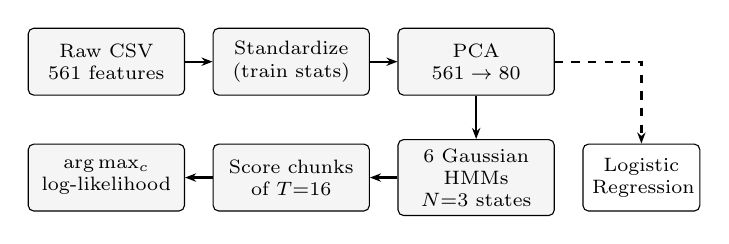
\begin{tikzpicture}[
  box/.style={draw, rounded corners=2pt, align=center, font=\scriptsize, minimum height=0.85cm, text width=1.75cm, fill=gray!8},
  arr/.style={-{Stealth[length=4pt]}, thick}]
\node[box] (a) {Raw CSV\\561 features};
\node[box, right=0.35cm of a] (b) {Standardize\\(train stats)};
\node[box, right=0.35cm of b] (c) {PCA\\$561\!\rightarrow\!80$};
\node[box, below=0.55cm of c] (d) {6 Gaussian HMMs\\$N{=}3$ states};
\node[box, left=0.35cm of d] (e) {Score chunks\\of $T{=}16$};
\node[box, left=0.35cm of e] (f) {$\arg\max_c$\\log-likelihood};
\draw[arr] (a) -- (b); \draw[arr] (b) -- (c); \draw[arr] (c) -- (d);
\draw[arr] (d) -- (e); \draw[arr] (e) -- (f);
\node[box, right=0.35cm of d, text width=1.25cm, fill=white] (g) {Logistic\\Regression};
\draw[arr, dashed] (c.east) -| (g.north);
\end{tikzpicture}
\caption{Pipeline. All transforms and models are fitted on training subjects only. The dashed branch is the per-window baseline.}
\label{fig:pipeline}
\end{figure}

\subsection{Preprocessing and Dimensionality Reduction}
Let $\mathbf{x}_t\in\mathbb{R}^{561}$ be the feature vector of window $t$. The activity label and the subject identifier are removed from the feature matrix. Using the subject identifier as a feature would let a model memorize individuals instead of motion patterns. Each feature is standardized with the mean and standard deviation of the training set. Principal component analysis~\cite{jolliffe2002pca} is then fitted on the standardized training data and applied unchanged to the test data, giving $\mathbf{o}_t=\mathbf{W}^\top(\mathbf{x}_t-\boldsymbol{\mu})/\boldsymbol{\sigma}\in\mathbb{R}^{d}$ with $d=80$. The 80 components retain 92.6\% of the training variance. Fitting either transform on test data would leak test information into the model. Fig.~\ref{fig:pca} shows the first two components. Static and dynamic activities separate clearly, while sitting and standing overlap.

\begin{figure}[t]
\centering
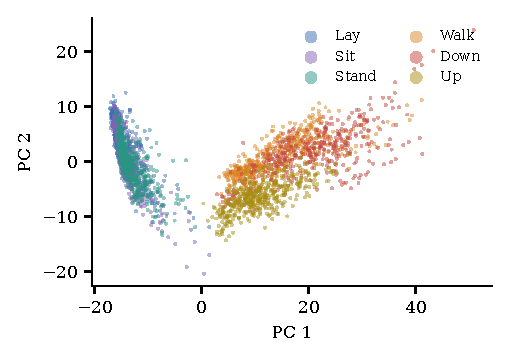
\includegraphics[width=0.95\columnwidth]{figures/pca.pdf}
\caption{Test windows in the first two principal components, colored by true activity.}
\label{fig:pca}
\end{figure}

\subsection{Class-Conditional Gaussian HMMs}
For each activity $c$, an HMM $\lambda_c=(\boldsymbol{\pi}_c,\mathbf{A}_c,\{\boldsymbol{\mu}_{c,i},\boldsymbol{\Sigma}_{c,i}\})$ with $N$ hidden states is trained. Here $\boldsymbol{\pi}_c$ is the initial state distribution, $\mathbf{A}_c$ the $N\times N$ transition matrix with $a_{ij}=P(s_{t+1}{=}j\mid s_t{=}i)$, and each state emits a Gaussian $\mathcal{N}(\boldsymbol{\mu}_{c,i},\boldsymbol{\Sigma}_{c,i})$ with diagonal covariance (variance floor $10^{-3}$). The likelihood of a sequence $O=\mathbf{o}_{1:T}$ is
\begin{equation}
P(O\mid\lambda_c)=\sum_{s_{1:T}}\pi_{c,s_1}\,b_{c,s_1}(\mathbf{o}_1)\prod_{t=2}^{T}a^{(c)}_{s_{t-1}s_t}\,b_{c,s_t}(\mathbf{o}_t),
\end{equation}
which the forward algorithm evaluates in $O(TN^2)$ time~\cite{rabiner1989tutorial}. The parameters are estimated by Baum--Welch (expectation--maximization)~\cite{baum1970maximization} for up to 100 iterations. The training sequences for class $c$ are the contiguous runs of that activity within each subject, and their lengths are passed to the learner so that no transition is learned across a run boundary. Treating every window as an independent one-step sequence would reduce the HMM to a Gaussian mixture and discard its temporal structure.

\subsection{Decision Rule and Segmentation}
Each test subject's stream is cut into consecutive chunks of $T=16$ windows (about 22\,s), never crossing a subject boundary. Every window in a chunk receives the label
\begin{equation}
\hat{c}=\arg\max_{c}\;\log P(\mathbf{o}_{t:t+T-1}\mid\lambda_c).
\end{equation}
The chunk length is the key design choice. Longer chunks give the transition model more context, but they are more likely to span an activity change.

\subsection{Baseline}
A multinomial Logistic Regression (L2 penalty, $C=1$, L-BFGS, 1,000 iterations) is trained on the same 80-dimensional features and classifies each window independently. It shows how much a conventional discriminative classifier achieves with identical inputs.

\section{Experimental Setup}
The pipeline is implemented in Python with scikit-learn~\cite{pedregosa2011scikit} (1.9) and hmmlearn~\cite{hmmlearn} (0.3.3), with random seed 42. Results are reported as accuracy, per-class precision, recall and F1, and macro-averaged F1 on all 2,947 test windows. The repository contains a command-line pipeline, a script that downloads the official UCI archive, an experiment script that regenerates every number and figure in this paper, a synthetic-data unit test and a continuous-integration workflow. On an Apple-silicon laptop, fitting all six HMMs and the baseline takes about 1.0\,s, and scoring the full test set takes 0.06\,s.

\section{Results}

\subsection{Main Comparison}
Table~\ref{tab:main} and Fig.~\ref{fig:confusion} compare the two models. The baseline is better on every class. The HMM's errors fall into two groups. The static postures are confused with one another: 124 of 532 standing windows are labeled as sitting, 116 of 491 sitting windows are mislabeled (67 as standing and 49 as laying), and 62 laying windows are labeled as sitting. The three walking activities are confused with one another, most notably 109 downstairs windows labeled as upstairs. Both models find the sitting--standing pair the hardest, which matches the overlap in Fig.~\ref{fig:pca}.

\begin{table}[t]
\caption{Test results with default settings ($d{=}80$, $N{=}3$, $T{=}16$)}
\label{tab:main}
\centering
\begin{tabular}{lcccc}
\toprule
& \multicolumn{2}{c}{HMM} & \multicolumn{2}{c}{Logistic Reg.} \\
\cmidrule(lr){2-3}\cmidrule(lr){4-5}
Activity & Recall & F1 & Recall & F1 \\
\midrule
Laying & 0.812 & 0.831 & 0.981 & 0.990 \\
Sitting & 0.764 & 0.703 & 0.872 & 0.878 \\
Standing & 0.739 & 0.789 & 0.914 & 0.902 \\
Walking & 0.857 & 0.857 & 0.972 & 0.945 \\
Downstairs & 0.664 & 0.683 & 0.907 & 0.930 \\
Upstairs & 0.786 & 0.761 & 0.904 & 0.909 \\
\midrule
Macro F1 & \multicolumn{2}{c}{0.771} & \multicolumn{2}{c}{0.926} \\
Accuracy & \multicolumn{2}{c}{77.3\%} & \multicolumn{2}{c}{92.6\%} \\
\bottomrule
\end{tabular}
\end{table}

\begin{figure*}[t]
\centering
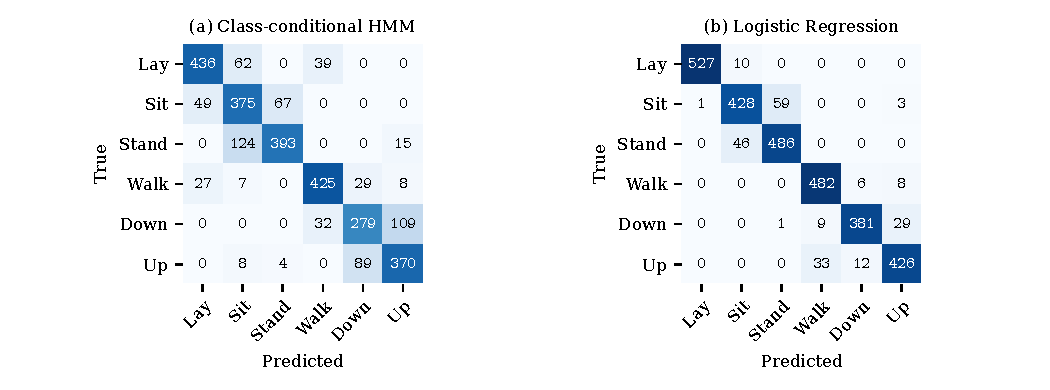
\includegraphics[width=0.82\textwidth]{figures/confusion.pdf}
\caption{Confusion matrices on the test set (window counts; shading is row-normalized). Rows are true activities and columns are predictions.}
\label{fig:confusion}
\end{figure*}

\begin{figure*}[t]
\centering
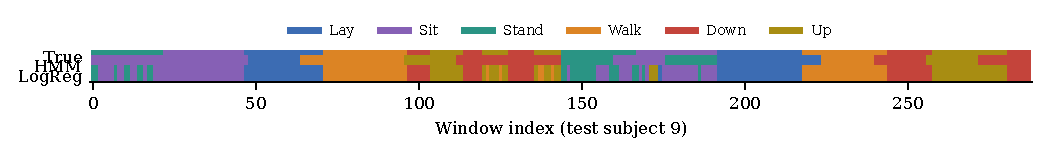
\includegraphics[width=0.92\textwidth]{figures/timeline.pdf}
\caption{True activities and predictions over time for test subject 9. HMM errors occur in blocks of 16 windows at activity changes. Logistic Regression errors are scattered single windows.}
\label{fig:timeline}
\end{figure*}

\subsection{Where the Gap Comes From}
Table~\ref{tab:diag} isolates the effect of segmentation. With fixed 16-window chunks, 100 of the 187 test chunks (53\%) contain more than one activity, because the average test run is only 24.6 windows long. A mixed chunk receives a single label, so part of it is wrong by construction. Three controlled variants make this clear:
\begin{itemize}
\item \emph{Single windows} ($T=1$): the same trained HMMs reach 85.5\%, more than eight points above the default.
\item \emph{Activity-aligned chunks}: when chunks of up to 16 windows are cut at the true activity boundaries, the same HMMs reach 92.0\% (macro F1 0.919). That is within 0.7 points of the baseline, with perfect recall and precision on walking. This variant uses ground-truth boundaries, so it is an upper bound for a segmenter, not a deployable method.
\item \emph{Chunk voting for the baseline}: giving every window in a fixed chunk the baseline's majority label drops its accuracy from 92.6\% to 81.5\%.
\end{itemize}
The baseline loses 11 points from the same chunking, which confirms that the segmentation, not the generative model, causes most of the gap. The difference between single windows (85.5\%) and aligned chunks (92.0\%) also shows that temporal context does help the HMM when a chunk covers one activity.

\begin{table}[t]
\caption{Segmentation diagnostics (same trained models)}
\label{tab:diag}
\centering
\begin{tabular}{llcc}
\toprule
Model & Test segmentation & Acc. & Macro F1 \\
\midrule
HMM & fixed chunks, $T{=}16$ (default) & 77.3\% & 0.771 \\
HMM & single windows, $T{=}1$ & 85.5\% & 0.854 \\
HMM & activity-aligned chunks$^\dagger$ & 92.0\% & 0.919 \\
LogReg & per window (default) & 92.6\% & 0.926 \\
LogReg & majority vote, $T{=}16$ & 81.5\% & 0.810 \\
\bottomrule
\multicolumn{4}{l}{\footnotesize $^\dagger$Uses ground-truth boundaries: an upper bound, not deployable.}
\end{tabular}
\end{table}

\subsection{Ablations}
Fig.~\ref{fig:ablation} varies the number of hidden states and the chunk length. Accuracy rises from 74.5\% with one state (a single Gaussian per class) to 78.9\% with four states and falls slightly with five. Chunk length matters far more. Accuracy is 85.5--85.9\% for $T\le4$, then falls to 83.6\% ($T{=}8$), 77.3\% ($T{=}16$), 66.5\% ($T{=}32$) and 39.4\% ($T{=}64$) as more chunks straddle activity changes. Table~\ref{tab:pca} varies the PCA dimension. Both models improve as more variance is kept, but the baseline gains more, from 84.0\% to 94.4\%, against 72.9\% to 78.2\% for the HMM. The diagonal-covariance Gaussians cannot exploit the extra dimensions as efficiently.

\begin{figure}[t]
\centering
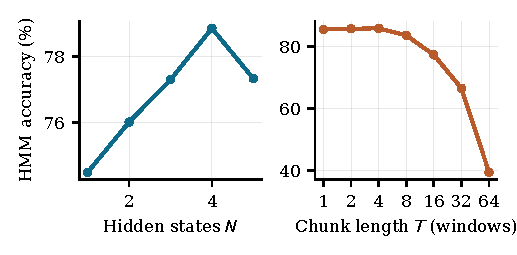
\includegraphics[width=\columnwidth]{figures/ablation.pdf}
\caption{HMM test accuracy versus the number of hidden states (left, $T{=}16$) and the test chunk length (right, $N{=}3$).}
\label{fig:ablation}
\end{figure}

\begin{table}[t]
\caption{Effect of the PCA dimension $d$ ($N{=}3$, $T{=}16$)}
\label{tab:pca}
\centering
\begin{tabular}{rccc}
\toprule
$d$ & Variance kept & HMM acc. & LogReg acc. \\
\midrule
10 & 70.8\% & 72.9\% & 84.0\% \\
20 & 77.4\% & 73.8\% & 87.5\% \\
40 & 85.0\% & 75.7\% & 90.1\% \\
80 & 92.6\% & 77.3\% & 92.6\% \\
160 & 98.5\% & 78.2\% & 94.4\% \\
\bottomrule
\end{tabular}
\end{table}

\subsection{Learned Dynamics and Per-Subject Variation}
The learned transition matrices are strongly persistent: the self-transition probabilities $a_{ii}$ range from 0.38 to 1.00 and are mostly above 0.75. The hidden states therefore last several windows and represent sub-phases of an activity rather than window-to-window noise. Accuracy varies widely across the nine test subjects, from 65.3\% to 87.2\% for the HMM and from 81.6\% to 97.6\% for the baseline. This shows that between-person variation in posture and gait remains a major challenge even for the stronger model. Fig.~\ref{fig:timeline} shows test subject 9, the HMM's weakest case. The HMM errors cluster at activity changes, where whole chunks take the label of the neighboring activity.


\section{Discussion and Limitations}
The study supports a clear conclusion. On UCI HAR, a class-conditional HMM with fixed-length segmentation is limited mainly by the segmentation, not by its probabilistic model. With chunks aligned to activity boundaries it nearly matches a strong per-window classifier, and temporal context then adds about 6.5 points over single-window scoring. Two properties of the data explain why the per-window baseline is hard to beat. First, each feature vector already summarizes 2.56\,s of signal with hand-crafted statistics, so most of the discriminative information sits inside a single window. Second, the test activity runs are short (about 31\,s on average), so long chunks often mix activities.

The study has limitations. The aligned-chunk result relies on ground-truth boundaries and only bounds what an ideal segmenter could reach. The temporal order of rows within a subject is assumed to match recording order. Only one dataset and one feature set were studied, and postural transitions are not modeled~\cite{reyesortiz2016transition}. Finally, the class-conditional design scores each activity independently and has no model of how one activity follows another.

\section{Conclusion and Future Work}
This paper presented a reproducible, leakage-free benchmark of class-conditional Gaussian HMMs for smartphone activity recognition. With the default 16-window chunks, the HMM reaches 77.3\% accuracy against 92.6\% for a Logistic Regression baseline. Diagnostics show that most of the gap comes from chunks spanning activity changes. Shorter chunks raise the HMM to 85.9\%, and boundary-aligned chunks to 92.0\%. Future work will remove the need for a fixed segmentation by joining the six activity models into one composite HMM with learned inter-activity transitions and decoding the whole stream with the Viterbi algorithm~\cite{viterbi1967error}, which segments and classifies at the same time. A hybrid that smooths discriminative per-window probabilities with an HMM, and evaluation on raw inertial signals and further datasets, are also planned.

\begin{thebibliography}{99}

\bibitem{lara2013survey}
O.~D. Lara and M.~A. Labrador, ``A survey on human activity recognition using wearable sensors,'' \emph{IEEE Commun. Surveys Tuts.}, vol.~15, no.~3, pp.~1192--1209, 2013.

\bibitem{bulling2014tutorial}
A.~Bulling, U.~Blanke, and B.~Schiele, ``A tutorial on human activity recognition using body-worn inertial sensors,'' \emph{ACM Comput. Surv.}, vol.~46, no.~3, pp.~33:1--33:33, 2014.

\bibitem{rabiner1989tutorial}
L.~R. Rabiner, ``A tutorial on hidden {M}arkov models and selected applications in speech recognition,'' \emph{Proc. IEEE}, vol.~77, no.~2, pp.~257--286, 1989.

\bibitem{anguita2013public}
D.~Anguita, A.~Ghio, L.~Oneto, X.~Parra, and J.~L. Reyes-Ortiz, ``A public domain dataset for human activity recognition using smartphones,'' in \emph{Proc. Eur. Symp. Artif. Neural Netw. (ESANN)}, Bruges, Belgium, 2013, pp.~437--442.

\bibitem{reyesortiz2016transition}
J.-L. Reyes-Ortiz, L.~Oneto, A.~Sam{\`a}, X.~Parra, and D.~Anguita, ``Transition-aware human activity recognition using smartphones,'' \emph{Neurocomputing}, vol.~171, pp.~754--767, 2016.

\bibitem{ronao2016human}
C.~A. Ronao and S.-B. Cho, ``Human activity recognition with smartphone sensors using deep learning neural networks,'' \emph{Expert Syst. Appl.}, vol.~59, pp.~235--244, 2016.

\bibitem{baum1970maximization}
L.~E. Baum, T.~Petrie, G.~Soules, and N.~Weiss, ``A maximization technique occurring in the statistical analysis of probabilistic functions of {M}arkov chains,'' \emph{Ann. Math. Statist.}, vol.~41, no.~1, pp.~164--171, 1970.

\bibitem{viterbi1967error}
A.~J. Viterbi, ``Error bounds for convolutional codes and an asymptotically optimum decoding algorithm,'' \emph{IEEE Trans. Inf. Theory}, vol.~13, no.~2, pp.~260--269, 1967.

\bibitem{kaufman2012leakage}
S.~Kaufman, S.~Rosset, C.~Perlich, and O.~Stitelman, ``Leakage in data mining: Formulation, detection, and avoidance,'' \emph{ACM Trans. Knowl. Discov. Data}, vol.~6, no.~4, pp.~15:1--15:21, 2012.

\bibitem{jolliffe2002pca}
I.~T. Jolliffe, \emph{Principal Component Analysis}, 2nd~ed. New York, NY, USA: Springer, 2002.

\bibitem{pedregosa2011scikit}
F.~Pedregosa \emph{et al.}, ``Scikit-learn: Machine learning in {P}ython,'' \emph{J. Mach. Learn. Res.}, vol.~12, pp.~2825--2830, 2011.

\bibitem{hmmlearn}
hmmlearn developers, ``hmmlearn: Hidden {M}arkov models in {P}ython, with scikit-learn like {API},'' 2024. [Online]. Available: \url{https://github.com/hmmlearn/hmmlearn}

\end{thebibliography}

\end{document}
